\chapter{High-Level Design}
\label{ch:high-level-design}

\section{Design intent}

The high-level design separates four concerns:

\begin{enumerate}
  \item \textbf{Catalog} --- what screens exist and what they need (data only).
  \item \textbf{Engine} --- how a recipe becomes files (pure transformation).
  \item \textbf{Clients} --- how a developer reaches the engine (I/O and UX).
  \item \textbf{Delivery} --- how catalog and packages reach the developer (build
        and CI).
\end{enumerate}

This separation is what allows the same recipe to be rendered by a terminal
program and by an editor extension with identical results.

\section{End-to-end generation flow}

\begin{figure}[H]
\centering
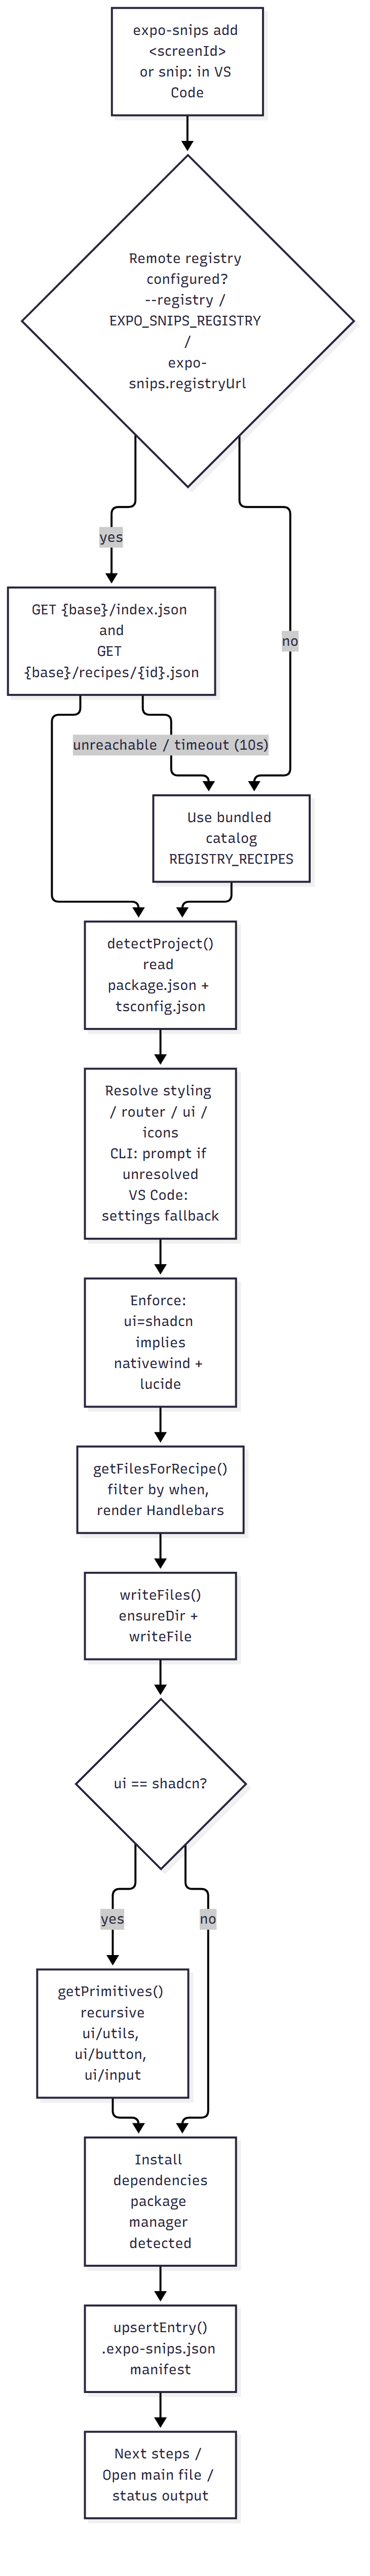
\includegraphics[width=\textwidth]{diagrams/generation-pipeline.png}
\caption{High-level generation pipeline from command to persisted manifest}
\label{fig:generation-pipeline}
\end{figure}

The pipeline has seven stages, each implemented in a single, identifiable place:

\begin{longtable}{@{}L{1cm}L{3.8cm}L{9.2cm}@{}}
\caption{Pipeline stages}\\
\toprule
\textbf{\#} & \textbf{Stage} & \textbf{Implementation} \\
\midrule
\endfirsthead
\toprule
\textbf{\#} & \textbf{Stage} & \textbf{Implementation} \\
\midrule
\endhead
1 & Resolve input & Parse the screen id and flags; fetch or select the recipe
(\texttt{add.ts}, \texttt{registry.ts}). \\
2 & Detect environment & Read \texttt{package.json} / \texttt{tsconfig.json}
(\texttt{detectProject.ts}). \\
3 & Resolve options & Apply precedence rules and prompts; enforce shadcn
constraints (\texttt{add.ts}). \\
4 & Render & Filter file entries by \texttt{when}; select template; compile with
Handlebars (\texttt{core/src/generate.ts}). \\
5 & Persist files & Create directories and write content
(\texttt{writeFiles.ts}). \\
6 & Resolve primitives & Recursively emit shadcn primitives, skipping existing
files (\texttt{primitives.ts}). \\
7 & Finalise & Install dependencies and record the install
(\texttt{installDeps.ts}, \texttt{manifest.ts}). \\
\bottomrule
\end{longtable}

\section{Major services and how they communicate}

There are no long-running services. The system's ``services'' are libraries and
one static endpoint.

\begin{longtable}{@{}L{3.8cm}L{4.6cm}L{5.6cm}@{}}
\caption{Service-equivalent components and their interactions}\\
\toprule
\textbf{Component} & \textbf{Interaction style} & \textbf{Peer} \\
\midrule
\endfirsthead
\toprule
\textbf{Component} & \textbf{Interaction style} & \textbf{Peer} \\
\midrule
\endhead
Generation engine & In-process function calls & CLI client, extension client \\
Embedded catalog & In-memory module import & CLI client, extension client \\
Registry endpoint & HTTP GET, JSON, read-only & Both clients (optional) \\
Package manager & Child process / terminal text & CLI client, extension client \\
create-expo-app & Child process & CLI client \\
VS Code host & Extension API & Extension client \\
\bottomrule
\end{longtable}

\section{Data model at a high level}

\begin{itemize}
  \item \textbf{Recipe} --- identity, version, supported stacks, dependencies,
        file templates (with conditions and overrides), optional variants, tags and
        primitive references. Defined by \texttt{ScreenRecipe} in
        \texttt{core/src/types.ts} and constrained by \texttt{registry/schema.json}.
  \item \textbf{Catalog index entry} --- the recipe subset needed for browsing:
        id, name, description, version, typescript flag, tags, supported stacks.
  \item \textbf{Generated file} --- a path plus rendered content.
  \item \textbf{Manifest entry} --- the record that a recipe was installed into a
        project.
\end{itemize}

\section{Cross-cutting concerns}

\begin{longtable}{@{}L{3.6cm}L{10.4cm}@{}}
\caption{Cross-cutting concerns and their handling}\\
\toprule
\textbf{Concern} & \textbf{Handling} \\
\midrule
\endfirsthead
\toprule
\textbf{Concern} & \textbf{Handling} \\
\midrule
\endhead
Error reporting & Coloured console output (CLI); VS Code error/information messages (extension). Non-zero exit code on failure. \\
Configuration & CLI flags and \texttt{EXPO\_SNIPS\_REGISTRY}; six VS Code settings. No config files. \\
Logging & Untyped console output; no log levels or destinations. \\
Offline behaviour & Embedded catalog; graceful fallback on every network failure. \\
Versioning & Semver on recipes and packages; the manifest stores the installed recipe version. \\
Extensibility & New recipes and new templates require no code change; new options would require type, schema, CLI-choice and settings changes. \\
\bottomrule
\end{longtable}

\section{Design trade-offs}

\begin{longtable}{@{}L{4.6cm}L{4.4cm}L{5cm}@{}}
\caption{Principal design trade-offs}\\
\toprule
\textbf{Choice} & \textbf{Benefit} & \textbf{Cost} \\
\midrule
\endfirsthead
\toprule
\textbf{Choice} & \textbf{Benefit} & \textbf{Cost} \\
\midrule
\endhead
Templates in JSON (inlined) & Portable, dependency-free rendering; works offline and over HTTP. & Poor diffs and review ergonomics in the built registry; JSON escaping of large templates. \\
Handlebars & One dependency; familiar syntax; easy recipe authoring. & Unchecked at compile time; typos surface only at render time. \\
Option enforcement instead of validation & Simpler command code. & Silent reprioritisation of user choices when \texttt{ui=shadcn} is selected. \\
Unconditional file writes on \texttt{add} & Simple, predictable generation. & A pre-existing file at a recipe path is overwritten with no warning. \\
Duplicated detection logic in the extension & Avoids a shared dependency on CLI internals. & Two implementations can diverge. \\
\bottomrule
\end{longtable}
